\documentclass[11pt,a4paper]{article}

% ------------------------------------------------------------------ packages
\usepackage[T1]{fontenc}
\usepackage{lmodern}
\usepackage[margin=2.5cm]{geometry}
\usepackage{amsmath,amssymb}
\usepackage{siunitx}
\usepackage{booktabs}
\usepackage{longtable}
\usepackage{array}
\usepackage{graphicx}
\usepackage{xcolor}
\usepackage{tikz}
\usetikzlibrary{positioning}
\usepackage{url}
\usepackage[numbers,sort&compress]{natbib}
\usepackage[hidelinks]{hyperref}
\usepackage[capitalise,noabbrev]{cleveref}

% Figures: ../figures when compiled inside report/, figures/ when the folder
% is uploaded next to main.tex in Overleaf.
\graphicspath{{../figures/}{figures/}}

% ------------------------------------------------------------------ notation
\newcommand{\Hs}{H_{s}}
\newcommand{\Tp}{T_{p}}
\newcommand{\pct}[1]{#1\,\%}
\newcommand{\dagnote}{\textsuperscript{\dag}}
\newcommand{\vect}[1]{\boldsymbol{#1}}
\DeclareMathOperator*{\argmin}{arg\,min}
\DeclareMathOperator*{\argmax}{arg\,max}

\title{Sea state estimation from vessel motions on RV Gunnerus\\[2pt]
       \large Theory, design decisions and process of the first concept (TMR06)}
\author{\textit{Author name}}
\date{\today}

\begin{document}
\maketitle

\begin{abstract}
\noindent
This report describes a first concept for estimating the significant wave height $\Hs$ and
the peak period $\Tp$ from the measured heave and pitch motions of a vessel on dynamic
positioning (DP). The data come from 250 co-simulations of RV Gunnerus in the Open Simulation
Platform (OSP): head seas, long-crested JONSWAP waves, 20-minute records, with sensor noise
added afterwards. Three families of estimators are compared on the same spectra: (i) a
physics-based inversion through the motion response amplitude operators (RAOs), by spectral
division and by a parametric JONSWAP fit; (ii) data-driven regression on the log spectra by
partial least squares (PLS) and principal component regression (PCR); and (iii) a hybrid in
which PLS corrects the physics estimate, following Martens' Continuous, Interpretable,
Minimalistic Machine Learning (CIM-ML) and called the CIM hybrid. To avoid an overly optimistic physics result, the
inversion uses a different RAO set from the one the simulator used. Models were selected by
repeated five-fold cross-validation on 200 calibration runs and scored once on 50 hidden test
runs. The CIM hybrid is best, with a root-mean-square relative error of
\pct{1.94} in $\Hs$ and \pct{0.74} in $\Tp$ on the test runs, against \pct{4.25} and
\pct{2.12} for PLS alone and \pct{5.81} and \pct{0.95} for the physics fit alone. A robustness
study then rescored the frozen models on 400 further runs, in which the true vessel's heave and
pitch RAOs were scaled or shifted in frequency, and with other sensor noise levels. A frequency
shift of 3--5\,\% raises the CIM hybrid's $\Hs$ error to 3.9--6.7\,\%, about the level of the physics
fit, although it stays the most stable method. A change in sensor noise ruins the purely
data-driven models (PLS up to \pct{74} in $\Hs$), while the physics fit stays near \pct{5}. The
gain from the CIM hybrid is therefore tied to the RAO error and the noise level it was trained on.
\end{abstract}

\tableofcontents
\clearpage

% ==================================================================
\section{Introduction}
\label{sec:intro}
% ==================================================================

A ship responds to the waves it is exposed to, and its motions can be measured cheaply and
continuously with an inertial measurement unit. Using the vessel itself as a wave sensor,
the \emph{wave buoy analogy}, is therefore an attractive way to obtain on-site sea state
information for decision support, operability assessment and DP
control \citep{nielsen2006,nielsen2017,tannuri2003,brodtkorb2018}. The difficulty is that the
ship is a filter: its response to a wave depends strongly on the wave frequency and direction,
described by its motion RAOs. Estimating the sea state from the motions is therefore an
inverse problem, and its accuracy depends on how well the RAOs are known.

This first concept answers a narrow question under controlled conditions: \emph{how accurately
can $\Hs$ and $\Tp$ be estimated from 20 minutes of heave and pitch on a DP vessel in head seas,
and does combining the physics with a data-driven correction help?} The data are simulated so
that the true sea state is known exactly and every condition can be repeated. The simulator
is the OSP co-simulation of RV Gunnerus in the \texttt{ospdpsimpy} package \citep{ospdpsimpy}.

Three estimators are compared on identical inputs:
\begin{enumerate}
  \item \textbf{Physics inversion}: the motion spectra divided by $|H|^2$, or a JONSWAP
        spectrum fitted through the RAOs to the measured motion spectra. Nothing is fitted to
        the simulated runs.
  \item \textbf{Data-driven regression}: PLS and PCR from the log motion spectra to
        $\log \Hs$ and $\log \Tp$, trained on the calibration runs.
  \item \textbf{CIM hybrid}: the physics fit, corrected by a PLS model trained on its residuals.
\end{enumerate}
A second question is how much of any gain survives when the vessel or the sensor differs from
the one the models were trained on, as it will on a real ship whose loading changes.
\Cref{sec:robustness} answers it with frozen models, a perturbed ``true'' vessel and other
sensor noise levels.

\Cref{sec:theory} gives the theory behind each step, \cref{sec:process} the process as it is
implemented in the project repository, \cref{sec:decisions} the design decisions and the evidence
for them, and \cref{sec:results,sec:discussion} the results, including the robustness study, and
their interpretation.
\Cref{sec:limitations} lists the limitations, and \cref{sec:repro} explains how to reproduce
everything.

% ==================================================================
\section{Theory}
\label{sec:theory}
% ==================================================================

\subsection{Irregular waves as a sum of regular waves}
\label{sec:waves}

In linear wave theory an irregular, long-crested sea is modelled as a sum of regular wave
components with random phases \citep{faltinsen1990,sorensen2013,fossen2021}. At a fixed point
the surface elevation is
\begin{equation}
  \zeta(t) = \sum_{k=1}^{N} a_k \cos(\omega_k t - \varphi_k),
  \qquad \varphi_k \sim \mathcal{U}[0, 2\pi),
  \label{eq:superposition}
\end{equation}
where the amplitudes follow from the one-sided wave spectrum $S_\zeta(\omega)$ and the
frequency spacing $\Delta\omega$:
\begin{equation}
  a_k = \sqrt{2\, S_\zeta(\omega_k)\, \Delta\omega}.
  \label{eq:amplitude}
\end{equation}
Each component contributes $a_k^2/2 = S_\zeta(\omega_k)\Delta\omega$ to the variance, so the
variance of $\zeta$ is the zeroth spectral moment
\begin{equation}
  m_n = \int_0^\infty \omega^n S_\zeta(\omega)\, d\omega,
  \qquad
  \operatorname{Var}\zeta = m_0 .
\end{equation}
The two quantities estimated in this work are the significant wave height and the peak period,
\begin{equation}
  \Hs = 4\sqrt{m_0},
  \qquad
  \Tp = \frac{2\pi}{\omega_p},
  \qquad
  \omega_p = \argmax_\omega S_\zeta(\omega).
  \label{eq:hs_tp}
\end{equation}
The simulator generates the waves exactly as in
\cref{eq:superposition,eq:amplitude}: the amplitudes are deterministic, and only the phases (and
a random offset of each frequency inside its bin) depend on the random seed. As a result, the
realised wave height varies far less between seeds than it would with Rayleigh-distributed
amplitudes in a real sea (see \cref{sec:limitations}).

\subsection{The JONSWAP spectrum}
\label{sec:jonswap}

Both the simulated waves and the parametric inversion use the JONSWAP
spectrum \citep{hasselmann1973} with the normalisation recommended by
DNV \citep{dnv2021c205}. It is the modified Pierson--Moskowitz spectrum
\begin{equation}
  S_{PM}(\omega) = \frac{5}{16}\, \Hs^2\, \omega_p^4\, \omega^{-5}
                   \exp\!\left[-\frac{5}{4}\left(\frac{\omega_p}{\omega}\right)^{4}\right]
  \label{eq:pm}
\end{equation}
multiplied by a peak enhancement:
\begin{equation}
  S_J(\omega) = A_\gamma\, S_{PM}(\omega)\,
                \gamma^{\exp\left[-\frac{(\omega-\omega_p)^2}{2\sigma^2\omega_p^2}\right]},
  \qquad
  A_\gamma = 1 - 0.287\ln\gamma,
  \qquad
  \sigma =
  \begin{cases}
    0.07, & \omega \le \omega_p,\\
    0.09, & \omega > \omega_p.
  \end{cases}
  \label{eq:jonswap}
\end{equation}
The factor $A_\gamma$ keeps the area close to $\Hs^2/16$ for any $\gamma$, and $\gamma = 1$ gives
back \cref{eq:pm}. The spectrum depends on three parameters, $(\Hs, \Tp, \gamma)$, and scales
exactly with $\Hs^2$:
\begin{equation}
  S_J(\omega; \Hs, \Tp, \gamma) = \Hs^2\, s(\omega; \Tp, \gamma),
  \label{eq:hs_scaling}
\end{equation}
where $s$ is the spectral shape for unit wave height. \Cref{sec:regression} uses this property.
The motion spectra are estimated per hertz, so the spectrum is converted as
$S(f) = 2\pi\, S(\omega)\big|_{\omega = 2\pi f}$.

A realistic sea is limited by wave breaking. The design (\cref{sec:step1}) limits the
peak steepness
\begin{equation}
  s_p = \frac{2\pi \Hs}{g \Tp^2} = \frac{\Hs}{\lambda_p} \le \frac{1}{15},
  \label{eq:steepness}
\end{equation}
where $\lambda_p = g\Tp^2/(2\pi)$ is the deep-water wavelength at the peak period.

\subsection{Linear vessel response}
\label{sec:rao}

For small motions the vessel is a linear, time-invariant system. The response of degree of
freedom $j$ to a single regular wave of unit amplitude, frequency $\omega$ and relative heading
$\beta$ is described by the complex motion RAO $H_j(\omega, \beta)$, computed by a panel
code \citep{faltinsen1990}. By superposition, the wave-frequency (WF) motion caused by the
wave train \cref{eq:superposition} is
\begin{equation}
  x_j(t) = \operatorname{Re}\Big\{ \sum_{k=1}^{N} \overline{H_j(\omega_k, \beta)}\,
            a_k\, e^{\,i(\omega_k t - \varphi_k)} \Big\},
  \label{eq:wf}
\end{equation}
which is the formula the vessel model of the simulator uses
(\path{src/ospfmusim/hull/helpfunctions/WF.py} in \texttt{ospdpsimpy}).
For a stationary Gaussian sea the response spectrum follows directly:
\begin{equation}
  S_{x_j}(\omega) = |H_j(\omega, \beta)|^2\, S_\zeta(\omega).
  \label{eq:response}
\end{equation}
For short-crested seas the right-hand side becomes an integral over directions, but in this
work the waves are long-crested and come from ahead ($\beta = 180^\circ$, head seas).
Three properties are used in what follows:
\begin{itemize}
  \item \textbf{Zero speed.} On DP the vessel holds its position, so the encounter frequency
        equals the wave frequency and no Doppler correction is needed.
  \item \textbf{Long-wave limits.} For waves much longer than the hull, the vessel follows the
        surface: $|H_{\text{heave}}| \to 1$ and $|H_{\text{pitch}}| \to k = \omega^2/g$
        (the wave slope, in rad/m). The implementation checks both limits.
  \item \textbf{Symmetry.} In head seas the port--starboard symmetry of the hull makes the roll
        RAO zero, so roll carries no information about the waves.
\end{itemize}
The simulator splits the motion into a low-frequency (LF) part, driven by slowly varying forces
and the DP thrusters, and the WF part \cref{eq:wf}. The DP controller acts on an LF estimate
from an extended Kalman filter with wave filtering, so the thrusters do not try to counteract
the first-order wave motion \citep{fossen2021,sorensen2013}. Heave and pitch are not controlled
at all, so their WF part is the sea state signal.

\subsection{Spectral estimation: Welch's method}
\label{sec:welch}

The motion spectra are estimated from a finite, sampled record $x[n] = x(n\Delta t)$ with
Welch's method \citep{welch1967}. The record is split into $M$ overlapping segments of $L$
samples. Each segment is detrended (mean removed), multiplied by a window $w[n]$ (Hann), and
transformed. The one-sided periodogram of segment $m$ is
\begin{equation}
  P_m(f) = \frac{2\Delta t}{\sum_n w[n]^2}
           \Big| \sum_{n=0}^{L-1} w[n]\, x_m[n]\, e^{-i 2\pi f n \Delta t} \Big|^2,
\end{equation}
and the estimate is the average $\hat S_x(f) = \frac{1}{M}\sum_m P_m(f)$. Three properties
matter here:
\begin{itemize}
  \item \textbf{Resolution.} The frequency bins are spaced $\Delta f = 1/(L\Delta t)$. A longer
        segment resolves narrower peaks, but gives fewer segments to average.
  \item \textbf{Variance.} Each periodogram value is approximately $\chi^2$-distributed with two
        degrees of freedom. Averaging $M$ segments (more with overlap) reduces the relative
        variance roughly as $1/M_{\text{eff}}$. The error is \emph{multiplicative}, which is
        why the fits and the regressions below work with the logarithm of the spectrum.
  \item \textbf{Leakage.} The expected value of the estimate is the true spectrum convolved
        with the power response of the window,
        \begin{equation}
          \operatorname{E}\big[\hat S_x(f)\big] = \int K(f - \nu)\, S_x(\nu)\, d\nu,
          \qquad
          K(\nu) \propto |W(\nu)|^2,
          \quad \int K = 1,
          \label{eq:leakage}
        \end{equation}
        where $W$ is the Fourier transform of the window \citep{harris1978}. A narrow
        spectral peak is therefore spread over neighbouring bins.
\end{itemize}
Zero-mean white sensor noise with standard deviation $\sigma_n$, sampled every $\Delta t$, has
the one-sided density
\begin{equation}
  N = 2\sigma_n^2 \Delta t,
  \label{eq:noise}
\end{equation}
so the expected estimate of a noisy motion is \cref{eq:leakage} plus $N$.

\subsection{The inverse problem: from motion spectra to the sea state}
\label{sec:inverse}

\paragraph{Spectral division.}
Inverting \cref{eq:response} gives an estimate of the wave spectrum,
\begin{equation}
  \hat S_\zeta(f) = \frac{\hat S_x(f)}{|H(f, \beta)|^2},
  \qquad f \in \mathcal{F} = \{ f : |H(f)| > c \max |H| \},
  \label{eq:division}
\end{equation}
from which $\Hs = 4\sqrt{\sum_{\mathcal{F}} \hat S_\zeta \Delta f}$ and $\Tp = 1/f_{\text{peak}}$
follow. The division is ill-conditioned where $|H|$ is small: noise in $\hat S_x$ and errors
in $H$ are amplified by $1/|H|^2$. The floor $c$ (here $0.2$) excludes these bins. Its price
is that wave energy outside $\mathcal{F}$ is not seen at all. An error in the RAO propagates
directly: since $\Hs \propto 1/|H|$, an RAO that is $\varepsilon$ too large gives an $\Hs$ that
is about $\varepsilon$ too small. The peak period is limited by the bin resolution, since
$\Tp$ can only take the values $1/f_k$. The relative step between neighbouring values is
$\Delta f\,\Tp$, which is 3--11\,\% for $\Tp = 4$--$14$\,s with the settings used here.

\paragraph{Parametric fit.}
The fit instead assumes the JONSWAP shape and searches for the parameters whose
\emph{predicted} motion spectra best match the measured ones. The model includes every effect
the measurement contains: the RAO, the window leakage \cref{eq:leakage} and the noise floor
\cref{eq:noise}:
\begin{equation}
  M_j(f; \vect\theta) = \Big( K * \big[ |H_j|^2\, S_J(\cdot\,; \Hs, \Tp, \gamma) \big] \Big)(f) + N_j,
  \qquad
  \vect\theta = (\ln\Hs, \ln\Tp, \ln\gamma).
  \label{eq:model}
\end{equation}
The parameters are found by nonlinear least squares in log space, over the same bins as the
division and over one or more motions $j$:
\begin{equation}
  \hat{\vect\theta} = \argmin_{\vect\theta \in \Theta}
    \sum_j \sum_{f \in \mathcal{F}_j}
    \big[ \ln M_j(f; \vect\theta) - \ln \hat S_{x_j}(f) \big]^2 .
  \label{eq:fit}
\end{equation}
Log residuals suit the multiplicative Welch error, and they give the tails of the spectrum,
which span several decades, a fair weight. The box $\Theta$ bounds
$\Hs \in [0.05, 20]$\,m, $\Tp \in [2, 30]$\,s and $\gamma \in [1, 10]$. The problem is solved
with a trust-region reflective method, starting from the division estimate and $\gamma = 3.3$.
Including the leakage kernel $K$ matters for long, narrow peaks: without it, the fit widens the
model peak to match the smeared measurement, which shifts $\Tp$ (\cref{sec:decisions}).

\paragraph{The inverse crime.}
If the same model is used to generate synthetic data and to invert them, the inversion looks
far better than it would on real data, because the model error is exactly zero. This is known
as an \emph{inverse crime} \citep{kaipio2005}. To avoid it, the inversion here uses a different
RAO set for RV Gunnerus from the one the simulator used, so the physics method has a realistic,
unknown model error (\cref{sec:decisions}).

\paragraph{What the motion spectra cannot tell.}
By \cref{eq:response,eq:hs_scaling}, $S_{x_j} = |H_j|^2\, \Hs^2\, s(\omega; \Tp, \gamma)$. If the
true RAO amplitude of every motion is $g|H_j|$, the motion spectra are exactly those of the
nominal vessel in a sea of height $g\Hs$. No method that sees only the motion spectra can tell
the two apart, so a common gain error in the RAOs passes one to one into $\Hs$ and leaves $\Tp$
unchanged. A change in the \emph{shape} of the RAO, such as a shift of its natural frequencies
with loading, changes the motion spectra in a way no sea state can mimic exactly, and is in
principle partly observable. \Cref{sec:step7} tests both.

\subsection{Multivariate regression on the spectra}
\label{sec:regression}

\paragraph{Features and targets.}
Each run gives one row $\vect x \in \mathbb{R}^p$: the $\log_{10}$ Welch spectra of heave and
pitch over the analysed band, one after the other ($p = 92$). The targets are
$\vect y = (\ln\Hs, \ln\Tp)$. The logarithms are motivated by \cref{eq:response,eq:hs_scaling}:
\begin{equation}
  \log_{10} S_{x_j}(f) = 2\log_{10}\Hs + \log_{10}|H_j(f)|^2 + \log_{10} s(f; \Tp, \gamma),
  \label{eq:log_linear}
\end{equation}
so $\log\Hs$ enters every feature as the same additive term. It is a single linear direction
in feature space, and a linear model can recover it exactly (up to the noise floor, which breaks
\cref{eq:log_linear} where the signal is weak). $\Tp$ moves the shape $s$ along the frequency
axis, which is not linear in the features, so more latent components are needed for $\Tp$.
Log targets also make the squared error a relative error, which matches the metric used for
scoring.

\paragraph{Autoscaling.}
Each column of $\vect X$ and $\vect Y$ is centred and divided by its standard deviation. The
means and standard deviations are computed on the training rows only and then applied to the
rows being predicted, so nothing from those rows leaks into the model.

\paragraph{Principal component analysis and regression.}
With the singular value decomposition of the scaled feature matrix,
$\tilde{\vect X} = \vect U \vect\Sigma \vect V^{\mathsf T}$, the first $A$ columns of
$\vect V$ are the directions of largest variance, and the share of variance they hold is
$\sum_{a \le A}\sigma_a^2 / \sum_a \sigma_a^2$ \citep{jolliffe2002}. PCR regresses the
targets on the scores $\vect T_A = \tilde{\vect X}\vect V_A$:
\begin{equation}
  \vect B_{\text{PCR}} = \vect V_A \big(\vect T_A^{\mathsf T}\vect T_A\big)^{-1}
                         \vect T_A^{\mathsf T}\tilde{\vect Y}.
\end{equation}
The directions are chosen without looking at the targets. A direction of large variance can
therefore be useless for prediction, and a useful one can come late.

\paragraph{Partial least squares.}
PLS chooses each direction to maximise the covariance between the scores and the targets
\citep{wold2001,hastie2009}. For two targets at once (PLS2), the weight vector of component
$a$ is the first left singular vector of $\tilde{\vect X}_a^{\mathsf T}\tilde{\vect Y}$, which
is the vector the NIPALS iteration converges to. With scores $\vect t_a = \tilde{\vect X}_a
\vect w_a$, loadings $\vect p_a = \tilde{\vect X}_a^{\mathsf T}\vect t_a / (\vect t_a^{\mathsf T}
\vect t_a)$ and $\vect q_a = \tilde{\vect Y}^{\mathsf T}\vect t_a / (\vect t_a^{\mathsf T}
\vect t_a)$, the feature matrix is deflated, $\tilde{\vect X}_{a+1} = \tilde{\vect X}_a - \vect
t_a \vect p_a^{\mathsf T}$, and after $A$ components the regression coefficients are
\begin{equation}
  \vect B_{\text{PLS}} = \vect W \big(\vect P^{\mathsf T}\vect W\big)^{-1} \vect Q^{\mathsf T}.
\end{equation}
In both methods a new row is predicted as
$\hat{\vect y} = (\tilde{\vect x}\vect B) \odot \vect s_Y + \bar{\vect y}$, and with $A = 0$
the prediction is the training mean. With all $A = p$ components, and $\tilde{\vect X}$ of full
column rank, both PCR and PLS reduce to ordinary least squares. The implementation uses this as a check.

\subsection{CIM hybrid model}
\label{sec:hybrid}

The hybrid follows the Continuous, Interpretable, Minimalistic Machine Learning (CIM-ML)
approach of \citet{martens2025}: first model the known variation from domain knowledge, then let
a transparent, low-dimensional data-driven model learn only the systematic variation that this
knowledge misses. It is therefore called the CIM hybrid. It keeps the physics estimate as the
backbone and lets the data correct it:
\begin{equation}
  \ln \hat{\vect y} = \ln \hat{\vect y}_{\text{phys}} + \hat{\vect r}(\vect x),
  \qquad
  \vect r = \ln\vect y - \ln\vect y_{\text{phys}},
  \label{eq:hybrid}
\end{equation}
where $\hat{\vect r}$ is a PLS model from the log spectra to the residual of the physics fit.
With $A = 0$ components the correction is the mean log bias of the physics estimate. With more
components, the correction can depend on the shape of the spectrum, for instance on where the
energy lies relative to frequency bands where the RAO is wrong. The physics carries the
nonlinear structure (the peak position and the $\Hs$ scaling), so the data-driven part only has
to learn a smooth, systematic model error.

Of the three properties in CIM-ML, the model has two. It is \emph{interpretable}: the backbone
is the RAOs and the JONSWAP spectrum, and the correction is one additive term in log units. It
is \emph{minimalistic}: the correction is a PLS model with few components, and $A = 0$ is a plain
bias correction. It is not \emph{continuous}: CIM-ML keeps learning as new measurements arrive,
whereas the CIM hybrid is trained once on the calibration runs and then frozen. The name refers
to the approach it follows, not a complete CIM-ML implementation.

\subsection{Model selection and validation}
\label{sec:validation}

\paragraph{Error metric.}
For each run $i$ the relative error is $e_i = \hat y_i / y_i - 1$. Each method is scored by
the root-mean-square relative error $\sqrt{\overline{e^2}}$ and the bias $\bar e$, both in
percent.

\paragraph{Repeated $K$-fold cross-validation.}
The calibration runs are split at random into $K = 5$ folds. Each fold is predicted by a model
trained on the other four, for every number of components $A = 0, \dots, 40$. The split is
repeated with three seeds and the errors are averaged \citep{hastie2009}. The number of
components with the lowest summed error $\varepsilon_{\Hs}(A) + \varepsilon_{\Tp}(A)$ is chosen.
The spread of the error between seeds shows how much the result depends on the split. Because
the same error is used to choose $A$, the cross-validated error of the chosen model is slightly
optimistic.

\paragraph{Hold-out test set and bootstrap.}
An unbiased error needs data that played no part in any choice. A separate set of test runs is
therefore kept aside and scored once, with the models refitted on all calibration runs. The
uncertainty of the test error from the limited number of runs is given as a 95\,\% percentile
bootstrap interval over the runs, from 2000 resamples \citep{efron1993}.

\paragraph{Experimental design.}
The sea states are chosen by Latin hypercube sampling (LHS) \citep{mckay1979}. The range of
each input is split into $n$ equal strata and each stratum is sampled exactly once, which
spreads $n$ runs evenly over the input space with far fewer runs than a full grid.

% ==================================================================
\section{Process}
\label{sec:process}
% ==================================================================

The pipeline consists of seven scripts in the root of the project repository, run in order.
Steps 1--6 build and score the estimators, and step 7 tests the frozen models under conditions
they were not fitted to. All settings are in \path{config.py} (\cref{app:config}). \Cref{fig:pipeline} shows the data flow. Every script
except the first has a \texttt{--check} option that tests its calculation against known answers
and its output file against the inputs (\cref{tab:checks}).

\begin{figure}[htbp]
  \centering
  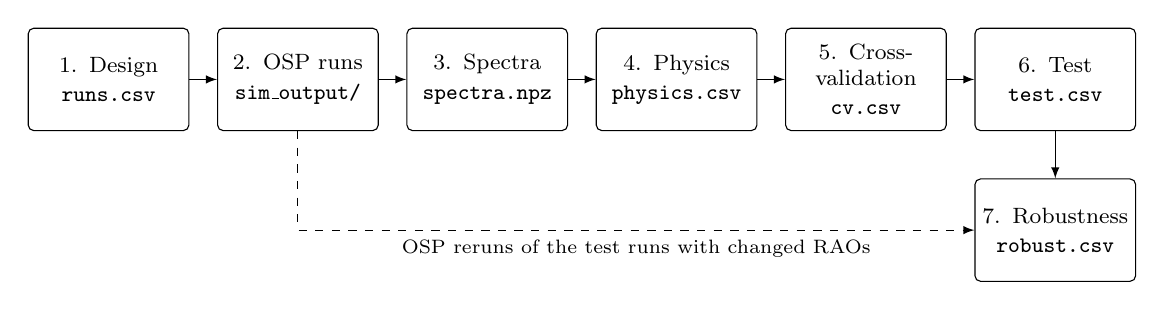
\begin{tikzpicture}[
      node distance=3.5mm,
      box/.style={draw, rounded corners=2pt, align=center, font=\footnotesize,
                  text width=19mm, minimum height=13mm, inner sep=2pt},
      >=latex]
    \node[box] (s1) {1. Design\\[1pt]\texttt{runs.csv}};
    \node[box, right=of s1] (s2) {2. OSP runs\\[1pt]\texttt{sim\_output/}};
    \node[box, right=of s2] (s3) {3. Spectra\\[1pt]\texttt{spectra.npz}};
    \node[box, right=of s3] (s4) {4. Physics\\[1pt]\texttt{physics.csv}};
    \node[box, right=of s4] (s5) {5. Cross-\\validation\\[1pt]\texttt{cv.csv}};
    \node[box, right=of s5] (s6) {6. Test\\[1pt]\texttt{test.csv}};
    \node[box, below=6mm of s6] (s7) {7. Robustness\\[1pt]\texttt{robust.csv}};
    \foreach \x/\y in {s1/s2, s2/s3, s3/s4, s4/s5, s5/s6, s6/s7}
      \draw[->] (\x) -- (\y);
    \draw[->, dashed] (s2.south) |- node[pos=0.75, below, font=\scriptsize]
      {OSP reruns of the test runs with changed RAOs} (s7.west);
  \end{tikzpicture}
  \caption{The seven steps and the file each one writes in \texttt{data/}. Steps 4--6 all read
           the spectra of step 3, and steps 5 and 6 also read the physics estimates of step 4.
           Step 7 reruns the test sea states in OSP with changed RAOs (dashed) and scores the
           frozen models of step 6 on them.}
  \label{fig:pipeline}
\end{figure}

\subsection{Simulation platform}
\label{sec:osp}

The runs are made with the OSP co-simulation of RV Gunnerus (length overall \SI{36.25}{m}) in
the \texttt{ospdpsimpy} package \citep{ospdpsimpy,osp,fmi2014}, which this project installs as a
dependency. The two are separate repositories, and the dependency is one-way: the simulator
knows nothing about sea state estimation, and this project only uses its FMUs and run tools,
its reader for the hydrodynamic data and its JONSWAP function. Each subsystem is a functional
mock-up unit (FMU):
\begin{itemize}
  \item a \textbf{wave} FMU that realises the spectrum as \cref{eq:superposition} with up to
        100 components;
  \item a \textbf{vessel} FMU with a six-degree-of-freedom LF model and the WF motion
        \cref{eq:wf}, both from the hydrodynamic data in \path{data_examples/gunnerus.mat};
  \item a \textbf{DP controller} (PID on surge, sway and yaw), an \textbf{extended Kalman
        filter} with wave filtering, \textbf{thrust allocation} and \textbf{thruster} models.
\end{itemize}
All constants not set per run are taken from \path{configs/gunnerus.toml}. Both paths are
inside the simulator repository.

\subsection{Step 1: experimental design}
\label{sec:step1}

\path{design_sea_states.py} draws a two-dimensional Latin hypercube in $(\Tp, u)$ with
$u \in [0,1]$ and maps $u$ to the wave height between the lower bound and an upper bound that
depends on $\Tp$:
\begin{equation}
  \Hs = H_{\min} + u\,\big(H_{\text{upper}}(\Tp) - H_{\min}\big),
  \qquad
  H_{\text{upper}}(\Tp) = \min\!\Big(H_{\max},\; \frac{1}{15}\frac{g\Tp^2}{2\pi}\Big).
\end{equation}
Every point is therefore realistic by \cref{eq:steepness}, and no samples are thrown away.
The steepness limit is active below $\Tp \approx \SI{6.2}{s}$. The calibration and test sets
are drawn with different seeds (\cref{tab:design}, \cref{fig:design}). Each run also gets its
own random wave seed. The design is written to \path{data/runs.csv}, one row per run, which is
the interface to the simulator.

\begin{table}[htbp]
  \centering
  \caption{Design of the sea states.}
  \label{tab:design}
  \begin{tabular}{@{}ll@{}}
    \toprule
    Setting & Value \\
    \midrule
    Calibration runs / test runs & 200 / 50 \\
    $\Hs$ range & 0.5--4.0\,m \\
    $\Tp$ range & 4--14\,s \\
    Maximum steepness $s_p$ & 1/15 \\
    JONSWAP $\gamma$ & 3.3 (fixed) \\
    Heading & $180^\circ$ (head seas) \\
    LHS seed, calibration / test & 1 / 3 \\
    Realised range, calibration & $\Hs$ 0.50--3.99\,m, $\Tp$ 4.02--13.96\,s \\
    Realised range, test & $\Hs$ 0.54--3.92\,m, $\Tp$ 4.16--13.90\,s \\
    \bottomrule
  \end{tabular}
\end{table}

\begin{figure}[htbp]
  \centering
  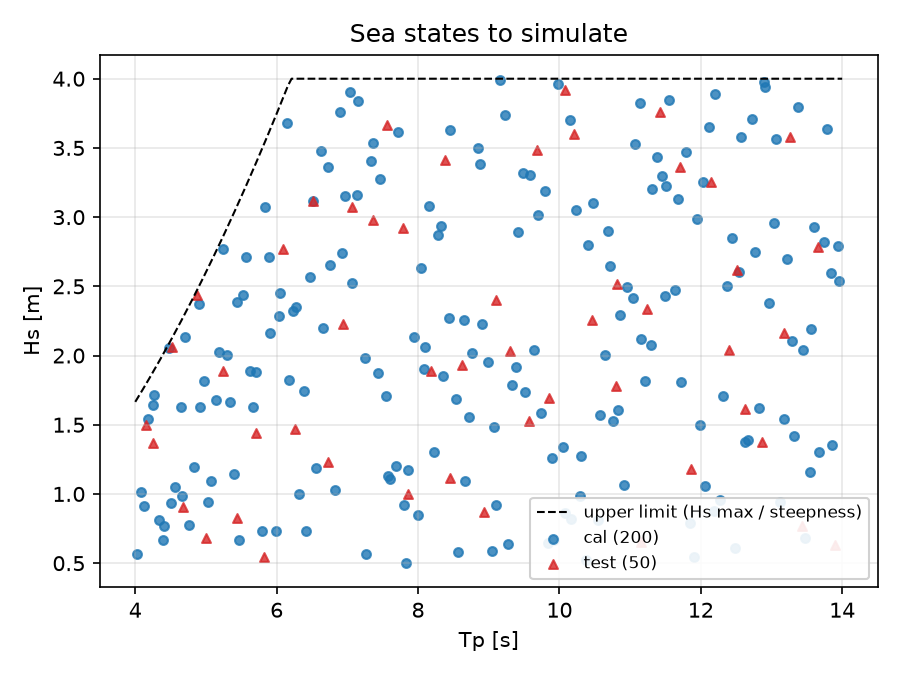
\includegraphics[width=0.62\textwidth]{design.png}
  \caption{The 250 sea states. The dashed line is the upper limit on $\Hs$, set by
           $H_{\max}$ and the steepness limit.}
  \label{fig:design}
\end{figure}

\subsection{Step 2: simulation in OSP}
\label{sec:step2}

\path{run_osp.py} runs every row of \path{runs.csv}. For each run it writes a configuration
file in which only the settings in \cref{tab:run_settings} differ from
\path{configs/gunnerus.toml}. The simulated time is a \SI{50}{s} ramp, which is discarded, plus
the analysed \SI{1200}{s} record, at a co-simulation step of \SI{0.5}{s}. The wave heading
relative to the bow is converted to the direction the waves come from in the north-east-down
frame, $\text{direction} = (\beta - 180^\circ + \psi_{\text{ref}}) \bmod 360^\circ$, which is
$0^\circ$ for head seas with the bow pointing north.

\begin{table}[htbp]
  \centering
  \caption{Settings changed per run from \texttt{configs/gunnerus.toml}.}
  \label{tab:run_settings}
  \begin{tabular}{@{}lll@{}}
    \toprule
    Setting & Value & Reason \\
    \midrule
    \texttt{waves.hs}, \texttt{tp}, \texttt{seed} & from \texttt{runs.csv} & the sea state \\
    \texttt{waves.direction\_deg} & $0^\circ$ & head seas \\
    \texttt{waves.spectrum.gamma} & 3.3 & JONSWAP \\
    \texttt{waves.spreading.type} & \texttt{none} & long-crested \\
    \texttt{waves.discretization.n\_frequencies} & 100 & all fit in the 100 wave outputs \\
    \texttt{waves.discretization.omega\_max\_factor} & $\Tp/2$ & grid top at $\pi$\,rad/s (\cref{sec:decisions}) \\
    \texttt{wind.enabled}, \texttt{current.enabled} & false & isolate the waves \\
    Vessel \texttt{max\_internal\_step\_s} & \SI{0.25}{s} & LF integration step \\
    \bottomrule
  \end{tabular}
\end{table}

The wave grid starts at $0.25\,\omega_p$ and ends at $\pi$\,rad/s (\SI{0.5}{Hz}), where the RAO
table of \path{gunnerus.mat} ends. Above that frequency the vessel model gives no response. Each
frequency is moved randomly inside its bin, so the wave groups do not repeat.

Each run is started in its own Python process, because an error inside an FMU ends the whole
process. Six runs are executed in parallel, a run that has produced no result after
\SI{600}{s} is stopped, and the output is written under a temporary name and renamed when
complete. A batch that stops can therefore simply be started again, and only the missing runs
are made. Instead of logging every variable to disk, a time-series observer in memory records
only the signals needed: heave, roll, pitch, the LF heading and position, and thruster
utilisation. The output is one CSV file per run, with heave in metres (positive down) and
angles in degrees.

All 250 runs completed, in 26 minutes and with \SI{48}{MB} of output. The check of the
analysed records found no thruster saturation. The worst values over all runs (each from a
different run) were a utilisation of 0.83, a heading deviation of $10.3^\circ$ and a position
offset of \SI{11.75}{m}.

\subsection{Step 3: motion spectra}
\label{sec:step3}

\path{build_spectra.py} keeps the analysed record ($t \ge t_{\text{ramp}}$, 2400 samples) of
each run and adds Gaussian white noise of \SI{0.02}{m} to heave and $0.02^\circ$ to pitch, to
represent the motion sensor. The noise is seeded per run, so it is the same every time.
It then computes one Welch spectrum per motion (\cref{tab:welch}). Bins outside
0.04--0.4\,Hz are dropped, since there the spectra are mostly sensor noise. The output
\path{data/spectra.npz} holds the spectra, the feature matrix $\vect X = \log_{10}$ spectra
($250 \times 92$), the targets and the split. $\vect X$ is not scaled in the file: scaling is
always fitted on training rows only. \Cref{fig:spectra} shows three calibration runs.

\begin{table}[htbp]
  \centering
  \caption{Spectral estimation settings.}
  \label{tab:welch}
  \begin{tabular}{@{}ll@{}}
    \toprule
    Setting & Value \\
    \midrule
    Record length / sample time & \SI{1200}{s} / \SI{0.5}{s} \\
    Segment length & \SI{128}{s} (256 samples), Hann window \\
    Overlap & 75\,\% (34 segments) \\
    Frequency resolution $\Delta f$ & $1/128 \approx \SI{7.8}{mHz}$ \\
    Band kept & 0.04--0.4\,Hz, 46 bins per motion \\
    Sensor noise $\sigma_n$ (assumed) & \SI{0.02}{m} heave, $0.02^\circ$ pitch \\
    Noise level $N$, \cref{eq:noise} & $4\times10^{-4}$\,m$^2$/Hz, $4\times10^{-4}$\,deg$^2$/Hz \\
    \bottomrule
  \end{tabular}
\end{table}

\begin{figure}[htbp]
  \centering
  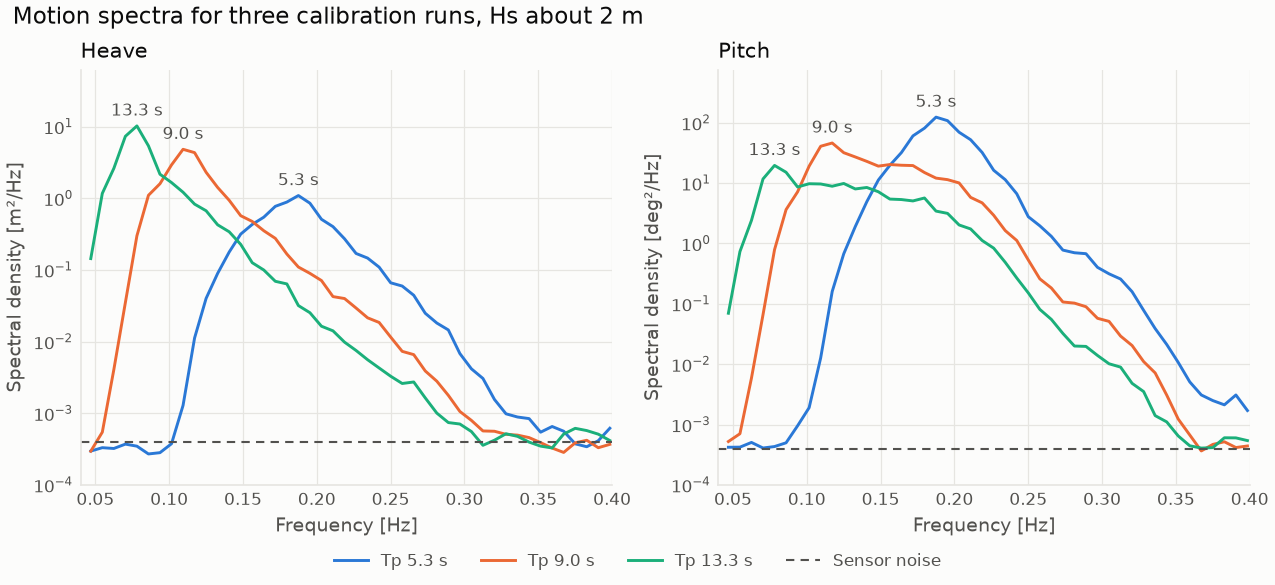
\includegraphics[width=\textwidth]{spectra.png}
  \caption{Heave and pitch spectra of three calibration runs with $\Hs \approx \SI{2}{m}$, from
           short to long waves, and the sensor noise level.}
  \label{fig:spectra}
\end{figure}

\subsection{Step 4: physics inversion}
\label{sec:step4}

\path{invert_spectra.py} estimates $\Hs$ and $\Tp$ for every run from its spectra alone, with
the RAOs of \path{GunnerusL35_20201112.mat} at $\beta = 180^\circ$ (pitch RAO converted to
deg/m). Five estimates are made per run:
\begin{itemize}
  \item \texttt{divide\_heave}, \texttt{divide\_pitch}: spectral division
        \cref{eq:division} with $c = 0.2$;
  \item \texttt{fit\_heave}, \texttt{fit\_pitch}: the fit \cref{eq:fit} to one motion;
  \item \texttt{fit\_all}: the fit to heave and pitch together.
\end{itemize}
The model \cref{eq:model} is evaluated on a grid eight times finer than the Welch bins, extended
by four bins on each side. It is convolved with the leakage kernel, which is the squared
magnitude of the zero-padded Fourier transform of the Hann window, normalised to unit sum, and
then sampled at the bins. The test runs are estimated as well, because the CIM hybrid model needs
them in step 6, but only the calibration runs are scored here. Nothing in this step is fitted to
the simulated runs.

\subsection{Step 5: cross-validation of PLS, PCR and the CIM hybrid}
\label{sec:step5}

\path{cross_validate.py} cross-validates three models on the 200 calibration runs only, as in
\cref{sec:validation}: PLS2 and PCR on $\vect X$, and the CIM hybrid \cref{eq:hybrid} with
\texttt{fit\_all} as the physics estimate. PLS and PCR are implemented in a few lines of NumPy
via the singular value decomposition. All scaling is fitted inside each training fold.
The error of every model for every number of components is written to \path{data/cv.csv}.

\subsection{Step 6: final evaluation}
\label{sec:step6}

\path{evaluate.py} refits each model on all 200 calibration runs with the number of components
chosen in step 5, predicts the 50 test runs, and scores these and the five physics estimates
once. It writes every estimate to \path{data/test.csv} and plots \cref{fig:cv,fig:test}. Its
check also confirms that each test run gets the same estimate when predicted alone as when
predicted with the others. That shows no statistic of the test runs (a mean or a scaling)
enters the models.

\subsection{Step 7: robustness to an unseen vessel or sensor}
\label{sec:step7}

The CIM hybrid of step 6 corrects one fixed RAO error, the one between
\path{GunnerusL35_20201112.mat} and \path{gunnerus.mat}, and the calibration and test runs share
it. On a real vessel the RAOs change with loading after a model has been trained, and the sensor
may not be the one assumed. \path{robustness.py} therefore freezes everything of step 6 (the
inversion RAOs, the models fitted on the calibration runs, their numbers of components, and the
sensor noise level assumed by the physics fit) and changes only the true vessel or the sensor:
\begin{itemize}
  \item \textbf{Gain}: heave and pitch $|H|$ of \path{gunnerus.mat} multiplied by
        $g \in \{0.90, 0.95, 1.05, 1.10\}$.
  \item \textbf{Shift}: heave and pitch RAO moved in frequency, $|H'(\omega)| = |H(\omega/s)|$,
        with $s \in \{0.95, 0.97, 1.03, 1.05\}$. The phase is kept, since only $|H|$ enters the
        spectra. The shift also scales the long-wave pitch RAO (the wave slope $k$) by $1/s^2$, so it
        stands in for a loading change rather than being a hull model. A draft change of
        6--10\,\% moves the natural periods by about 3--5\,\%.
  \item \textbf{Noise}: the sensor noise standard deviation set to 0, 0.05 and 0.10 (m for
        heave, degrees for pitch) instead of 0.02. No new runs are needed.
\end{itemize}
For each gain and shift, the script writes a copy of \path{gunnerus.mat} to \path{data/robust/} in
which only the motion RAO table is changed, so the DP system sees exactly the same loads. It then
reruns the 50 test sea states in OSP with that file (\texttt{run\_osp.py --mat ... --out ...},
about five minutes per file, 400 runs in all). Every condition uses the same sea states, wave
phases and noise draws (scaled), and the same bootstrap resamples, so a change in error is caused
by the perturbation alone. Nothing is chosen on these results, so the test runs may be scored
again. The control condition must reproduce \path{data/test.csv}, which the check confirms.

\begin{table}[htbp]
  \centering
  \caption{What each \texttt{--check} tests. All six pass on the delivered data.}
  \label{tab:checks}
  \small
  \begin{tabular}{@{}p{3.3cm}p{11.7cm}@{}}
    \toprule
    Script & Checks \\
    \midrule
    \texttt{run\_osp.py} & every output file exists, has the right time vector and finite
      motions; no thruster saturation; reports the worst DP utilisation, heading and offset \\
    \texttt{build\_spectra.py} & a sine peaks at its own frequency with area $A^2/2$; white
      noise gives $2\sigma^2\Delta t$; the file follows \texttt{runs.csv} \\
    \texttt{invert\_spectra.py} & long-wave RAO limits (heave $\to 1$, pitch $\to k$); JONSWAP
      area $= \Hs^2/16$; the leakage model reproduces Welch for a sine between two bins within
      2\,\%; a spectrum made with the model gives back its own $(\Hs,\Tp,\gamma)$ from every fit \\
    \texttt{cross\_validate.py} & PLS and PCR with all components equal ordinary least squares;
      one PLS component points along $\vect X^{\mathsf T}\vect y$ \\
    \texttt{evaluate.py} & \texttt{test.csv} matches a fresh estimate; no test run influences the
      estimate of another \\
    \texttt{robustness.py} & each changed \texttt{.mat} file differs from \texttt{gunnerus.mat}
      only in the heave and pitch $|H|$ (phase, loads and matrices unchanged); the control
      reproduces \texttt{test.csv}; a gain of 1.10 gives 1.10 times the $\Hs$ of
      \texttt{fit\_pitch} on every run (measured 1.0998) and the same $\Tp$, which proves OSP
      used the changed file \\
    \bottomrule
  \end{tabular}
\end{table}

% ==================================================================
\section{Design decisions}
\label{sec:decisions}
% ==================================================================

\Cref{tab:decisions} summarises the decisions made while building the pipeline, the alternative
that was rejected, and the evidence. Most numbers come from the delivered scripts and data.
Those marked \dagnote{} come from exploratory measurements made while the pipeline was being
designed. Their scripts are not part of the repository, so they should be re-measured
before they are relied on in a different setting. The most important decisions are then
discussed in more detail.

{\small
\setlength{\tabcolsep}{4pt}
\begin{longtable}{@{}>{\raggedright\arraybackslash}p{2.5cm}>{\raggedright\arraybackslash}p{3.4cm}>{\raggedright\arraybackslash}p{2.6cm}>{\raggedright\arraybackslash}p{6.4cm}@{}}
  \caption{Design decisions. \dagnote{} = exploratory measurement, not reproduced by the delivered scripts.}
  \label{tab:decisions}\\
  \toprule
  Decision & Choice & Rejected & Reason and evidence \\
  \midrule
  \endfirsthead
  \toprule
  Decision & Choice & Rejected & Reason and evidence \\
  \midrule
  \endhead
  \bottomrule
  \endfoot
  Data source & OSP co-simulation with DP & direct linear generator (spectrum $\times$ RAO) &
    Includes DP, LF motion and numerical integration. In head seas OSP adds only
    $\approx 0.3$ points of $\Hs$ error to PLS (\pct{4.24} against \pct{3.98}\dagnote). \\
  Sea condition & head seas, long-crested, no wind or current & oblique and short-crested seas &
    Judge the method before the DP complicates it. Head-sea heave and pitch match the linear RAO
    response (correlation $\ge 0.993$\dagnote). In beam seas ($\Hs = 3.5$\,m, $\Tp = 6.6$\,s) the
    DP saturated \pct{23.5} of the time, with heading error up to $20^\circ$ and roll up to
    $37^\circ$\dagnote. \\
  Motions used & heave and pitch & also roll &
    The head-sea roll RAO is zero. Measured roll is only a DP yaw artefact\dagnote. \\
  RAOs for inversion & \texttt{GunnerusL35\_20201112.mat} (runs use \texttt{gunnerus.mat}) &
    the same file & Avoids the inverse crime. The two RAO sets differ mostly below
    $T = 8$\,s\dagnote. With matched RAOs, \texttt{fit\_all} reaches \pct{1.49} / \pct{0.71} in
    $\Hs$ / $\Tp$ instead of \pct{6.18} / \pct{0.99}. \\
  Time step & \SI{0.5}{s}, LF step \SI{0.25}{s} & \SI{0.1}{s}; \SI{1}{s} &
    Variance within \pct{0.2} and spectra within 0.14\,dB of the \SI{0.1}{s} step, about five
    times faster\dagnote. A \SI{1}{s} step degraded the DP\dagnote. \\
  Data logging & in-memory observer, 7 signals & CSV of every variable &
    Estimated 25\,min and 40\,MB for 250 runs instead of 3\,h and 31\,GB\dagnote. Realised:
    26\,min, 48\,MB. \\
  Record length & \SI{1200}{s} + \SI{50}{s} ramp & \SI{300}{s} records &
    Records of \SI{300}{s} clearly increased the PLS error\dagnote. A \SI{50}{s} ramp is enough in
    head seas (\SI{200}{s} is suggested for oblique seas). \\
  Wave grid top & $\pi$\,rad/s for every $\Tp$ & default $3\,\omega_p$ &
    The default cut leaves a cliff of up to 30\,dB in the spectrum whose position gives away
    $\Tp$ (\cref{sec:dec_grid}). \\
  Sensor noise & \SI{0.02}{m}, $0.02^\circ$, added afterwards & none; noise inside OSP &
    A real sensor has a noise floor. Adding it afterwards lets the level change without new
    runs. The values are assumed, not taken from a data sheet. \\
  Welch settings & \SI{128}{s}, 75\,\%, 0.04--0.4\,Hz & other segment lengths &
    Balances resolution and variance. Tuned on calibration runs only. \\
  Log features and targets & $\log_{10} S$, $\ln\Hs$, $\ln\Tp$ & linear spectra &
    $\Hs$ becomes additive \cref{eq:log_linear}, the Welch error becomes additive, and the loss
    becomes relative. \\
  Physics estimator & JONSWAP fit with leakage kernel and noise floor & division only; fit
    without kernel; robust loss &
    Division is limited by the bin resolution and the band (\cref{sec:dec_fit}). Without the
    kernel $\Tp$ was biased $+\pct{3}$\dagnote. Soft-L1 and Cauchy losses left the heave bias at
    $+\pct{13}$\dagnote. \\
  RAO floor & $|H| > 0.2\max|H|$ & no floor &
    Below the floor, noise and relative RAO error are amplified by $1/|H|^2$. \\
  Hybrid base & \texttt{fit\_all} & \texttt{fit\_pitch} &
    Uses both motions and has the lowest $\Tp$ error on the calibration runs (\pct{0.99}); its
    $\Hs$ error is systematic and therefore learnable. \\
  Implementation & NumPy PLS2 and PCR via SVD & scikit-learn &
    Not installed in the environment, and a few lines each. Verified against least squares. \\
  Model selection & 5 folds $\times$ 3 seeds, $A = 0..40$, minimum of $\varepsilon_{\Hs} +
    \varepsilon_{\Tp}$ & single split & Seed spread $\le 0.07$ points for the CIM hybrid. 40
    components were needed to see the PCR minimum. \\
  Test set & 50 runs, LHS seed 3, scored once & seed 2 &
    The seed-2 runs were used to choose the simulation settings, so they were no longer hidden. \\
  Design & LHS in $(\Tp, u)$, steepness $\le 1/15$, $\gamma = 3.3$ & grid; rejection sampling &
    Even coverage with no discarded samples; every sea state is realistic. \\
  Robustness test & frozen models; true RAO scaled or shifted and rerun in OSP; noise changed &
    perturbing only the inversion RAOs; refitting per condition &
    PLS never sees an RAO, so only a change of the \emph{true} vessel tests it. Refitting would
    hide the effect of a loading change after training. Only the motion RAO table changes, so
    the DP loads are identical, and the phases and noise draws are shared. \\
\end{longtable}
}

\subsection{Different RAOs for generation and inversion}
\label{sec:dec_rao}

The most consequential decision is to invert with \path{GunnerusL35_20201112.mat} while the
simulator uses \path{gunnerus.mat}. Both describe RV Gunnerus, but they differ, mostly for
periods below about 8\,s. On real data the RAOs are never exact, so a physics method tested
with the generating RAOs would be flattered. With the generating RAOs, the fit to both motions
gives \pct{1.49} RMS error in $\Hs$ and \pct{0.71} in $\Tp$ on the calibration runs, and
recovers a median $\gamma$ of 3.30 against the true 3.3. With the other RAO file it gives
\pct{6.18} and \pct{0.99}. Almost all of the remaining physics error is therefore model error in
the RAOs, which is exactly the error the CIM hybrid model is meant to remove.

\subsection{Top of the wave grid}
\label{sec:dec_grid}

By default the wave FMU spans $0.25\,\omega_p$ to $3\,\omega_p$. The spectrum then drops by up
to 30\,dB at $3/\Tp$\,Hz. In the motion spectra this cliff falls inside the analysed band at a
position set by $\Tp$, so a regression can read $\Tp$ from the cliff rather than from the
physics. With the default grid, PLS chose 21 components and reached \pct{5.25} in $\Hs$ and
\pct{1.76} in $\Tp$\dagnote. With the grid top fixed at $\pi$\,rad/s it chose 8 components and
reached \pct{4.24} and \pct{2.31}\dagnote. The apparent $\Tp$ accuracy with the default grid
came from this leak. The top is set to $\pi$\,rad/s (\texttt{omega\_max\_factor} $= \Tp/2$)
because that is where the RAO table ends and the vessel response is zero. A lower top would only
remove real waves, since the number of components is capped at 100. At $\Tp \approx 4$\,s, up to
\pct{4.5} of the wave variance lies above $\pi$\,rad/s and is not generated. The vessel would not
respond to it anyway, so the motions are those of the full sea, and the nominal $\Hs$ remains
the correct target.

\subsection{The physics estimator}
\label{sec:dec_fit}

Division needs no assumption about the spectral shape, but it has two built-in limits. $\Tp$ can
only take the values $1/f_k$ of the Welch bins, a step of $\Delta f\,\Tp$ (3--11\,\%). $\Hs$ only
includes the energy inside the bins where the RAO is large enough. Both limits remain with
perfect RAOs: with the generating RAOs, division still gives \pct{5.46} (heave) and \pct{4.78}
(pitch) in $\Hs$ and 3.2--3.3\,\% in $\Tp$. The JONSWAP fit removes both limits by fitting a
continuous model, which extrapolates through the known shape. It must, however, model the
measurement completely. Without the leakage kernel, long-period peaks were matched by a model
peak that was too wide, which biased $\Tp$ by about $+\pct{3}$ and made the fitted $\gamma$
fall with $\Tp$\dagnote. The noise floor is included in the model rather than subtracted from
the data, which keeps the log residuals finite where the motion is weak.

% ==================================================================
\section{Results}
\label{sec:results}
% ==================================================================

\subsection{Physics inversion on the calibration runs}

\Cref{tab:physics_cal} gives the physics estimates on the 200 calibration runs, with the RAOs of
\path{GunnerusL35_20201112.mat}. No parameter is fitted to the runs, but the settings of the
method were chosen while looking at these runs, so the unbiased errors are the test values in
\cref{tab:test}. The joint fit is best for $\Tp$ (\pct{0.99}). The pitch fit is best for
$\Hs$ (\pct{4.80}) but is biased low, and the heave fit is strongly biased high. The median
$\gamma$ from \texttt{fit\_all} is 2.62, against a true value of 3.3.

\begin{table}[htbp]
  \centering
  \caption{Physics estimates on the 200 calibration runs: RMS relative error and bias [\%].}
  \label{tab:physics_cal}
  \begin{tabular}{@{}lrrrr@{}}
    \toprule
    & \multicolumn{2}{c}{$\Hs$} & \multicolumn{2}{c}{$\Tp$} \\
    \cmidrule(lr){2-3}\cmidrule(l){4-5}
    Method & RMS & bias & RMS & bias \\
    \midrule
    \texttt{divide\_heave} &  4.91 &  $+1.65$ & 3.95 & $-0.85$ \\
    \texttt{divide\_pitch} &  9.56 &  $-8.66$ & 3.30 & $+0.31$ \\
    \texttt{fit\_heave}    & 23.67 & $+15.22$ & 1.97 & $-1.66$ \\
    \texttt{fit\_pitch}    &  4.80 &  $-4.18$ & 1.13 & $-0.06$ \\
    \texttt{fit\_all}      &  6.18 &  $+2.84$ & 0.99 & $-0.63$ \\
    \bottomrule
  \end{tabular}
\end{table}

\subsection{Cross-validation}

Five components hold \pct{90} of the variance of the scaled calibration spectra, and 19 hold
\pct{99}. \Cref{tab:cv} and \cref{fig:cv} give the cross-validated error. With no components,
PLS and PCR predict the mean sea state (\pct{76.8} error in $\Hs$ and \pct{40.4} in $\Tp$), while the CIM hybrid with
no components, which is the physics fit with its mean bias removed, already gives \pct{5.38} and
\pct{0.78}. PLS reaches its minimum at 7 components. PCR needs 25 and improves slowly, as
expected for components chosen without regard to the targets. The CIM hybrid needs only 4.

\begin{table}[htbp]
  \centering
  \caption{Cross-validated RMS relative error [\%] on the calibration runs (5 folds, 3 seeds),
           at the chosen number of components $A$.}
  \label{tab:cv}
  \begin{tabular}{@{}lrrr@{}}
    \toprule
    Model & $A$ & $\Hs$ & $\Tp$ \\
    \midrule
    PLS    &  7 & 4.22 & 2.34 \\
    PCR    & 25 & 4.30 & 2.17 \\
    CIM hybrid &  4 & 1.76 & 0.71 \\
    \bottomrule
  \end{tabular}
\end{table}

\begin{figure}[htbp]
  \centering
  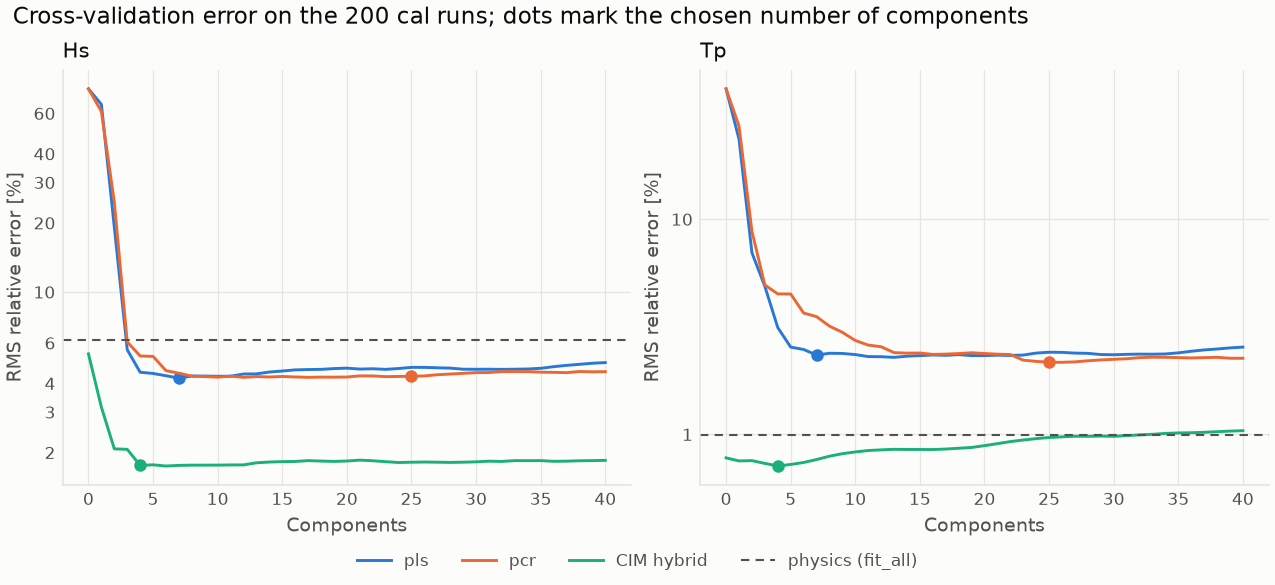
\includegraphics[width=\textwidth]{cv.png}
  \caption{Cross-validated error against the number of components. Dots mark the chosen
           number; the dashed line is the error of the physics fit \texttt{fit\_all}.}
  \label{fig:cv}
\end{figure}

\subsection{Test runs}

\Cref{tab:test} gives the single evaluation on the 50 hidden test runs, and \cref{fig:test}
shows the error of each test run against its true peak period. For every method and both
targets, the calibration value lies inside the 95\,\% interval of the test error, so the choices
made on the calibration runs did not overfit. The CIM hybrid has the lowest error in both $\Hs$ and
$\Tp$. Its interval for $\Hs$ (1.34--2.50\,\%) lies entirely below those of every other method.
For $\Tp$ its interval overlaps that of \texttt{fit\_all}, so on 50 runs the gain in $\Tp$ over the
physics fit is not significant.

\begin{table}[htbp]
  \centering
  \caption{Errors on the 50 test runs [\%]. \emph{Cal}: cross-validated error for the models,
           calibration-run error for the physics methods. \emph{Test}: RMS relative error,
           its 95\,\% bootstrap interval, and the mean (bias).}
  \label{tab:test}
  \small
  \setlength{\tabcolsep}{4pt}
  \begin{tabular}{@{}lrrrcrrrcr@{}}
    \toprule
    & & \multicolumn{4}{c}{$\Hs$} & \multicolumn{4}{c}{$\Tp$} \\
    \cmidrule(lr){3-6}\cmidrule(l){7-10}
    Method & $A$ & cal & test & 95\,\% interval & bias & cal & test & 95\,\% interval & bias \\
    \midrule
    \texttt{divide\_heave} & -- &  4.91 &  5.38 &  3.99--6.61  &  $+1.30$ & 3.95 & 3.75 & 3.13--4.36 & $-1.22$ \\
    \texttt{divide\_pitch} & -- &  9.56 &  9.62 &  8.25--10.98 &  $-8.65$ & 3.30 & 3.47 & 2.82--4.08 & $-0.06$ \\
    \texttt{fit\_heave}    & -- & 23.67 & 22.28 & 14.84--28.63 & $+14.75$ & 1.97 & 1.89 & 1.65--2.11 & $-1.69$ \\
    \texttt{fit\_pitch}    & -- &  4.80 &  4.79 &  4.28--5.34  &  $-4.28$ & 1.13 & 1.02 & 0.76--1.32 & $-0.02$ \\
    \texttt{fit\_all}      & -- &  6.18 &  5.81 &  3.99--7.44  &  $+2.71$ & 0.99 & 0.95 & 0.78--1.13 & $-0.67$ \\
    \midrule
    PLS                    &  7 &  4.22 &  4.25 &  3.23--5.22  &  $+0.30$ & 2.34 & 2.12 & 1.72--2.51 & $-0.20$ \\
    PCR                    & 25 &  4.30 &  3.96 &  3.01--4.84  &  $+0.35$ & 2.17 & 2.12 & 1.72--2.50 & $-0.13$ \\
    \textbf{CIM hybrid}    &  4 &  1.76 & \textbf{1.94} &  1.34--2.50 & $-0.11$ & 0.71 & \textbf{0.74} & 0.57--0.91 & $-0.04$ \\
    \bottomrule
  \end{tabular}
\end{table}

\begin{figure}[htbp]
  \centering
  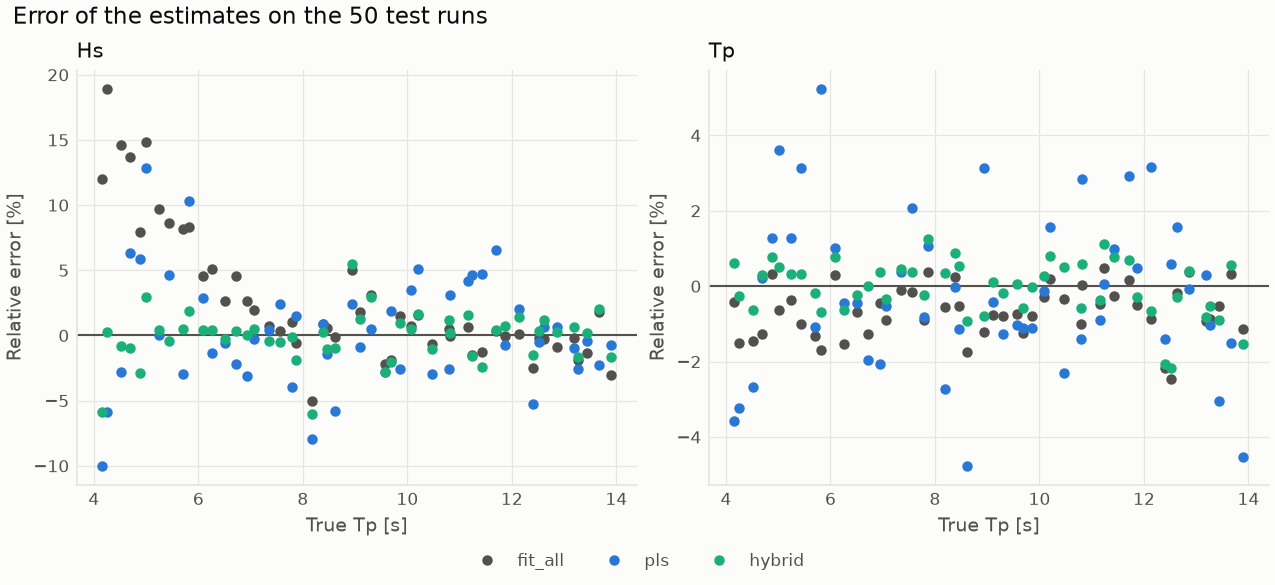
\includegraphics[width=\textwidth]{test.png}
  \caption{Relative error of each test run against its true $\Tp$, for the physics fit
           \texttt{fit\_all}, PLS and the CIM hybrid.}
  \label{fig:test}
\end{figure}

\subsection{Robustness to an unseen vessel or sensor}
\label{sec:robustness}

\Cref{tab:robust} and \cref{fig:robust} give the errors of the frozen models of step 6 on the test
runs when the true vessel or the sensor changes (\cref{sec:step7}). The control reproduces
\cref{tab:test} exactly.

\begin{table}[htbp]
  \centering
  \caption{RMS relative error [\%] on the 50 test runs when the true vessel or the sensor
           differs from the one the models were fitted to. The models and the inversion RAOs
           are those of step 6, and the control row is \cref{tab:test}.}
  \label{tab:robust}
  \small
  \setlength{\tabcolsep}{3.5pt}
  \begin{tabular}{@{}llrrrrrrrr@{}}
    \toprule
    & & \multicolumn{4}{c}{$\Hs$} & \multicolumn{4}{c}{$\Tp$} \\
    \cmidrule(lr){3-6}\cmidrule(l){7-10}
    Change & Level & \texttt{fit\_pitch} & \texttt{fit\_all} & PLS & CIM hybrid
                   & \texttt{fit\_pitch} & \texttt{fit\_all} & PLS & CIM hybrid \\
    \midrule
    Control          & --   &  4.79 &  5.81 &  4.25 &  1.94 & 1.02 & 0.95 &  2.12 & 0.74 \\
    \midrule
    Gain $g$         & 0.90 & 13.96 &  8.90 & 10.48 & 10.28 & 1.01 & 0.96 &  2.25 & 0.75 \\
                     & 0.95 &  9.28 &  5.48 &  6.25 &  5.44 & 1.01 & 0.96 &  2.17 & 0.74 \\
                     & 1.05 &  2.31 &  9.51 &  6.93 &  5.30 & 1.03 & 0.94 &  2.09 & 0.73 \\
                     & 1.10 &  5.78 & 14.15 & 11.40 & 10.14 & 1.03 & 0.94 &  2.10 & 0.73 \\
    \midrule
    Shift $s$        & 0.95 &  7.40 &  2.59 & 13.45 &  6.69 & 1.94 & 0.86 &  5.41 & 1.44 \\
                     & 0.97 &  5.55 &  2.40 &  8.33 &  4.36 & 1.43 & 0.69 &  3.41 & 1.04 \\
                     & 1.03 &  6.94 &  9.68 & 11.21 &  3.85 & 1.42 & 1.46 &  2.66 & 1.08 \\
                     & 1.05 &  9.29 & 12.15 & 16.96 &  6.00 & 1.97 & 1.80 &  3.23 & 1.50 \\
    \midrule
    Noise $\sigma_n$ & 0    &  4.74 &  6.42 & 28.43 &  7.93 & 1.03 & 1.24 & 18.34 & 4.56 \\
                     & 0.05 &  5.10 &  5.06 & 30.77 &  5.54 & 1.34 & 0.96 & 13.54 & 2.19 \\
                     & 0.10 &  5.86 &  5.20 & 74.47 & 10.51 & 2.52 & 2.69 & 26.77 & 3.32 \\
    \bottomrule
  \end{tabular}
\end{table}

\begin{figure}[htbp]
  \centering
  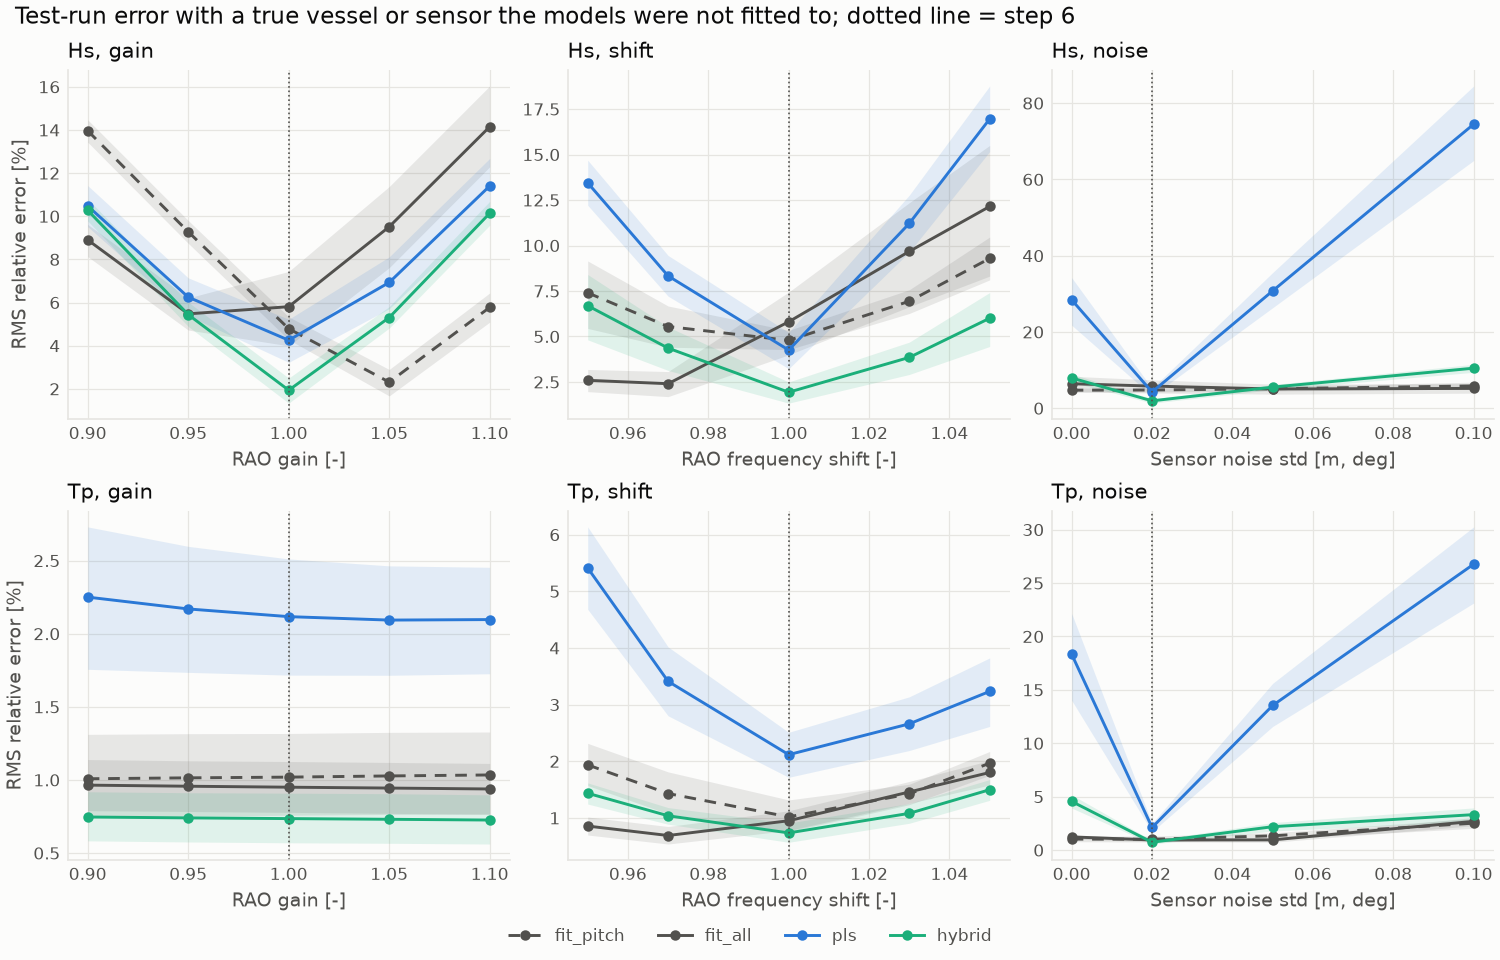
\includegraphics[width=\textwidth]{robust.png}
  \caption{Test-run RMS error against the size of each change, for the two physics fits, PLS and
           the CIM hybrid, with 95\,\% bootstrap intervals. The dotted line marks the condition of
           step 6. The vertical scales differ between panels.}
  \label{fig:robust}
\end{figure}

\paragraph{Gain.}
As \cref{sec:inverse} predicts, a common gain on the heave and pitch RAOs cannot be detected:
every method's $\Hs$ follows it, and $\Tp$ is untouched (CIM hybrid 0.73--0.75\,\%). The bias of the
CIM hybrid moves from $-0.1$\,\% to $-10.1$\,\% at $g = 0.90$ and to $+9.9$\,\% at $g = 1.10$, and
PLS behaves the same. No method amplifies the gain, so the CIM hybrid error is close to $|g - 1|$
itself. The physics fits, which start out biased, can be helped as well as hurt:
\texttt{fit\_pitch}, biased $-4.3$\,\% in the control, improves to \pct{2.31} at $g = 1.05$.

\paragraph{Frequency shift.}
A shift is the more realistic case, since loading moves the natural periods. Here the advantage
of the CIM hybrid shrinks. Its $\Hs$ error rises from \pct{1.94} to 3.9--6.7\,\%, and its $\Tp$ error
from \pct{0.74} to 1.0--1.5\,\%. PLS degrades most ($\Hs$ 8.3--17.0\,\%, $\Tp$ up to
\pct{5.4}), because it has learned where the spectral features of one particular vessel lie. The
physics fit reacts asymmetrically: \texttt{fit\_all} improves to 2.4--2.6\,\% for $s < 1$,
because the shift partly cancels the mismatch between the two RAO files, and rises to \pct{12.2}
at $s = 1.05$. Over the four shifts the CIM hybrid has the lowest worst case (\pct{6.7}, against
\pct{12.2} for \texttt{fit\_all} and \pct{17.0} for PLS) and the lowest mean (\pct{5.2}, against
\pct{6.7} and \pct{12.5}). Its accuracy of about \pct{2} in step 6 is, however, specific to the
RAO error it was trained on.

\paragraph{Sensor noise.}
A change of sensor noise hardly affects the physics fits ($\Hs$ 4.7--6.4\,\%, $\Tp$ at most
\pct{2.7}), even though the fit still assumes the nominal noise level. It ruins PLS: the $\Hs$
error is \pct{28} with no noise, \pct{31} at 0.05 and \pct{74} at 0.10, with $\Tp$ errors of
13--27\,\%. The PLS bias in $\Hs$ changes sign with the noise level ($-18.8$\,\% at
$\sigma_n = 0$, $+27.6$\,\% at 0.05 and $+68.0$\,\% at 0.10), so PLS reads the noise floor as
wave energy. Of all spectral bins of the 250 runs, \pct{36} of the heave bins and \pct{17} of
the pitch bins lie within a factor of three of the noise floor (\cref{fig:spectra}). In log scale
these bins weigh as much as the peak, so the models have learned the floor. The CIM hybrid inherits
the problem in a weaker form ($\Hs$ 5.5--10.5\,\%, $\Tp$ 2.2--4.6\,\%), because its PLS
correction reads the same bins.

% ==================================================================
\section{Discussion}
\label{sec:discussion}
% ==================================================================

\paragraph{Physics is best for the period, data for the height, and the CIM hybrid for both.}
The JONSWAP fit locates the spectral peak precisely (\pct{0.95} in $\Tp$ on the test runs),
because the period is set by the position of the peak, which a wrong RAO amplitude barely
moves. The wave height, in contrast, is inversely proportional to the RAO amplitude, so the RAO
error passes straight into $\Hs$. PLS has the opposite profile. $\Hs$ is a linear direction in
log feature space \cref{eq:log_linear}, while $\Tp$ requires several components to follow the
peak along the frequency axis. The CIM hybrid inherits the $\Tp$ accuracy of the physics, and its
PLS correction removes most of the $\Hs$ error. On the test runs it reaches \pct{1.94}, close to
the \pct{1.49} (calibration runs) of the physics fit with the \emph{correct} RAOs. In this setting, a few PLS components learn most of what the RAO
mismatch costs.

\paragraph{Where the physics error comes from.}
The biases in \cref{tab:physics_cal} are consistent with the known differences between the two
RAO files\dagnote. The pitch RAO of the L35 file is about \pct{7} higher than that of the
generating file at 0.08--0.2\,Hz, which predicts $\Hs$ about \pct{7} too low. The division from
pitch is \pct{8.7} low, and the pitch fit, which also uses the spectral shape, is \pct{4.2} low.
The heave RAO of the L35 file has a notch at 0.18--0.26\,Hz. There the measured heave has energy
that the model can only explain with larger waves, so the heave fit is \pct{15} high. These
frequencies hold the peak of short seas, so the physics error is concentrated at $\Tp < 6$\,s,
where \texttt{fit\_all} overestimates $\Hs$ by up to about \pct{19} on single runs
(\cref{fig:test}). The CIM hybrid removes this pattern. The fitted $\gamma$ (median 2.62 instead of
3.3) is a symptom of the same mismatch: with the generating RAOs the fit recovers 3.30.

\paragraph{The simulator adds little error in head seas.}
PLS on the OSP data (\pct{4.24} in $\Hs$) is close to PLS on data from a direct linear generator
without DP (\pct{3.98}\dagnote). In head seas the DP loop, the LF motion and the numerical
integration add only about 0.3 points of error. This is consistent with the near-perfect
correlation between OSP heave and pitch and the linear RAO response\dagnote.

\paragraph{The evaluation is sound.}
The test set was drawn with its own seed, never used for any choice, and scored once. Every
calibration value lies inside the 95\,\% interval of the corresponding test error, and the
leakage check confirms that no test statistic enters the models. With 50 test runs the interval
spans between about $\pm$10\,\% and $\pm$30\,\% of the error itself. Differences smaller than
that, such as between PLS and PCR, are not significant.

\paragraph{The CIM hybrid learns one RAO error, not RAO errors in general.}
The robustness study qualifies the main result. The PLS correction of the CIM hybrid learns the
specific mismatch between the two RAO files, which the calibration and test runs share. When the
true vessel moves by 3--5\,\% in frequency, the CIM hybrid falls back to roughly the accuracy of the
physics fit (3.9--6.7\,\% in $\Hs$), although it stays the most stable method across the shifts.
A common gain error is invisible to every method and passes straight into $\Hs$, so the absolute
level of the RAOs must come from elsewhere, for instance a model test or a calibration against a
wave buoy. The noise result is a warning for any data-driven model on log spectra: it must be
trained at the noise level of the actual sensor, or its features must be made insensitive to it,
for example by clipping the log spectra at a fixed multiple of the noise floor or by training on
several noise levels. The physics fit avoids the problem because it models the noise floor
explicitly and only uses bins where the RAO is large, which mostly lie well above the floor.

% ==================================================================
\section{Limitations and further work}
\label{sec:limitations}
% ==================================================================

\begin{itemize}
  \item \textbf{Simulated data only.} The motions are linear by construction (\cref{eq:wf}),
        and the true sea state is the nominal one. On a real vessel, non-linear responses,
        RAO errors of unknown size, and the reference measurement itself add error.
  \item \textbf{Optimistic sampling variability.} The wave amplitudes are deterministic
        (\cref{sec:waves}), so the realised $\Hs$ of a 20-minute record varies only
        0.3--2.7\,\% between seeds\dagnote. In a real sea the sampling variability of a
        20-minute record is larger, and the errors reported here are therefore a lower bound.
  \item \textbf{Narrow conditions.} Head seas only, long-crested, zero speed, no wind or current,
        unimodal JONSWAP with fixed $\gamma = 3.3$. The data-driven models have never seen
        another $\gamma$, swell or bimodal seas, and are not expected to extrapolate to them.
  \item \textbf{Assumed sensor noise.} \SI{0.02}{m} and $0.02^\circ$ are assumed values, to be
        replaced by the data sheet of the actual motion sensor. Step 7 shows that the
        data-driven models depend strongly on this value (PLS 28--74\,\% in $\Hs$ when it
        changes), so they must be trained at the real level.
  \item \textbf{One RAO pair.} The CIM hybrid learns the difference between two specific RAO files,
        and step 7 shows that most of its gain is lost when the true RAOs shift by 3--5\,\%. On a
        real vessel it would need training data with a reference sea state (a wave buoy or a
        calibrated simulator) that covers the loading conditions in operation.
  \item \textbf{Not continuous.} The CIM hybrid is fitted once and then frozen, so it lacks the
        continuous learning of CIM-ML \citep{martens2025}. Step 7 shows the cost: when the
        vessel changes, nothing in the model updates.
  \item \textbf{Perturbations are stand-ins.} The gains and shifts of step 7 change heave and pitch
        together and uniformly over frequency. A real loading change alters the RAO shape in a
        more complicated way and also changes the DP loads.
  \item \textbf{Test set spent.} The 50 test runs have been used to score the models of step 6
        and, without any tuning, the frozen models of step 7. They must not be used for further
        tuning. A new comparison needs new test runs.
\end{itemize}
Natural next steps are oblique and short-crested seas, where roll must be added back and the
relative wave direction becomes a third target, and where DP heading wander becomes important.
Step 7 points to two more: features that are insensitive to the noise floor (clipped log spectra
or training on several noise levels), and training the CIM hybrid over a range of RAO perturbations,
so that it learns a family of RAO errors rather than a single one. Updating the correction as
new data arrive would add the missing continuous part of CIM-ML. Others are varying $\gamma$
and bimodal seas, forward speed (encounter frequency), validation on full-scale Gunnerus data
with a reference buoy, and an uncertainty estimate per prediction.

% ==================================================================
\section{Reproducibility}
\label{sec:repro}
% ==================================================================

All results can be reproduced from the project repository. It needs the simulator next to it:
\begin{enumerate}
  \item Check out \texttt{ospdpsimpy} \citep{ospdpsimpy} next to the project folder, as
        \path{../ospdpsimpy} (\texttt{SIM\_REPO} in \path{config.py}).
  \item Put \path{gunnerus.mat} and \path{GunnerusL35_20201112.mat} in
        \path{../ospdpsimpy/data_examples/}. They are not in git.
  \item Make a Python 3.11 virtual environment in the project folder and install
        \path{requirements.txt}, which installs \texttt{ospdpsimpy} as an editable package.
\end{enumerate}
Then run the commands below from the repository root. The OSP output (\path{data/sim_output/}
and \path{data/robust/}, about \SI{124}{MB}) is not in git, but the results of steps 3--7 are.
Steps 3--6 take seconds to minutes and do not need OSP. Step 2 takes about 26 minutes with six
parallel runs, and step 7 about 40 minutes (eight RAO files of 50 runs each).

\begin{verbatim}
python design_sea_states.py   # 1: data/runs.csv, figures/design.png
python run_osp.py             # 2: data/sim_output/ (restartable)
python build_spectra.py       # 3: data/spectra.npz, figures/spectra.png
python invert_spectra.py      # 4: data/physics.csv
python cross_validate.py      # 5: data/cv.csv
python evaluate.py            # 6: data/test.csv, figures/cv.png, test.png
python robustness.py          # 7: data/robust/, data/robust.csv, robust.png
\end{verbatim}
Each script except the first accepts \texttt{--check} (\cref{tab:checks}), and all six pass on the
delivered data.

\bibliographystyle{plainnat}
\bibliography{references}

\appendix
% ==================================================================
\section{All settings}
\label{app:config}
% ==================================================================

\begin{table}[htbp]
  \centering
  \caption{Settings in \texttt{config.py}.}
  \label{tab:config}
  \small
  \begin{tabular}{@{}lll@{}}
    \toprule
    Name & Value & Meaning \\
    \midrule
    \texttt{N\_CAL}, \texttt{N\_TEST} & 200, 50 & calibration and test runs \\
    \texttt{HS\_RANGE} & 0.5--4.0\,m & significant wave height \\
    \texttt{TP\_RANGE} & 4--14\,s & peak period \\
    \texttt{MAX\_STEEPNESS} & 1/15 & $2\pi\Hs/(g\Tp^2)$ \\
    \texttt{GAMMA} & 3.3 & JONSWAP peak enhancement \\
    \texttt{HEADINGS\_DEG} & 180 & head seas \\
    \texttt{DESIGN\_SEED\_CAL}, \texttt{\_TEST} & 1, 3 & LHS seeds \\
    \texttt{DURATION\_S} & 1200\,s & analysed record \\
    \texttt{RAMP\_S} & 50\,s & discarded start-up \\
    \texttt{DT\_S} & 0.5\,s & co-simulation step and sample time \\
    \texttt{MAX\_INTERNAL\_STEP\_S} & 0.25\,s & LF integration step \\
    \texttt{N\_WORKERS} & 6 & parallel runs \\
    \texttt{MOTIONS} & heave, pitch & signals used \\
    \texttt{WELCH\_SEGMENT\_S} & 128\,s & Welch segment \\
    \texttt{WELCH\_OVERLAP} & 0.75 & segment overlap \\
    \texttt{FREQ\_RANGE\_HZ} & 0.04--0.4\,Hz & band kept \\
    \texttt{SENSOR\_NOISE\_STD} & 0.02\,m, 0.02$^\circ$ & assumed sensor noise \\
    \texttt{NOISE\_SEED} & 1 & noise seed \\
    \texttt{INVERSION\_MAT} & \texttt{GunnerusL35\_20201112.mat} & RAOs for inversion \\
    \texttt{N\_FOLDS} & 5 & cross-validation folds \\
    \texttt{CV\_SEEDS} & 0, 1, 2 & fold seeds \\
    \texttt{MAX\_COMPONENTS} & 40 & largest $A$ tried \\
    \texttt{SIM\_REPO} & \path{../ospdpsimpy} & simulator repository \\
    \texttt{TRUE\_MAT} & \texttt{gunnerus.mat} & RAOs the runs were made with \\
    \texttt{RAO\_GAINS} & 0.90, 0.95, 1.05, 1.10 & step 7: heave and pitch $|H|$ times $g$ \\
    \texttt{RAO\_SHIFTS} & 0.95, 0.97, 1.03, 1.05 & step 7: heave and pitch $|H(\omega/s)|$ \\
    \texttt{NOISE\_LEVELS} & 0, 0.05, 0.10 & step 7: sensor noise std [m, deg] \\
    \midrule
    \multicolumn{3}{@{}l}{\emph{Fixed in the scripts}} \\
    \texttt{RAO\_FLOOR} & 0.2 & bins used: $|H| > 0.2\max|H|$ \\
    \texttt{GAMMA\_START} & 3.3 & start value of the fit \\
    \texttt{OVERSAMPLE}, \texttt{REACH} & 8, 4 & fine grid per bin; kernel half-width in bins \\
    \texttt{HYBRID\_BASE} & \texttt{fit\_all} & physics estimate corrected by the CIM hybrid \\
    \texttt{N\_BOOTSTRAP} & 2000 & bootstrap resamples \\
    \bottomrule
  \end{tabular}
\end{table}

\end{document}
